
\begin{frame}{Applications}
  \begin{outline}
    \1 Giga-voxel topology optimization on a single machine \cite{Liu2018}

    % Complexity of Sparse data structures
    % Freedom to explore this space
    % Add Figure 4 somewhere
  \end{outline}
\end{frame}

\begin{frame}{Life of a Taichi Kernel}
  \begin{centering}
    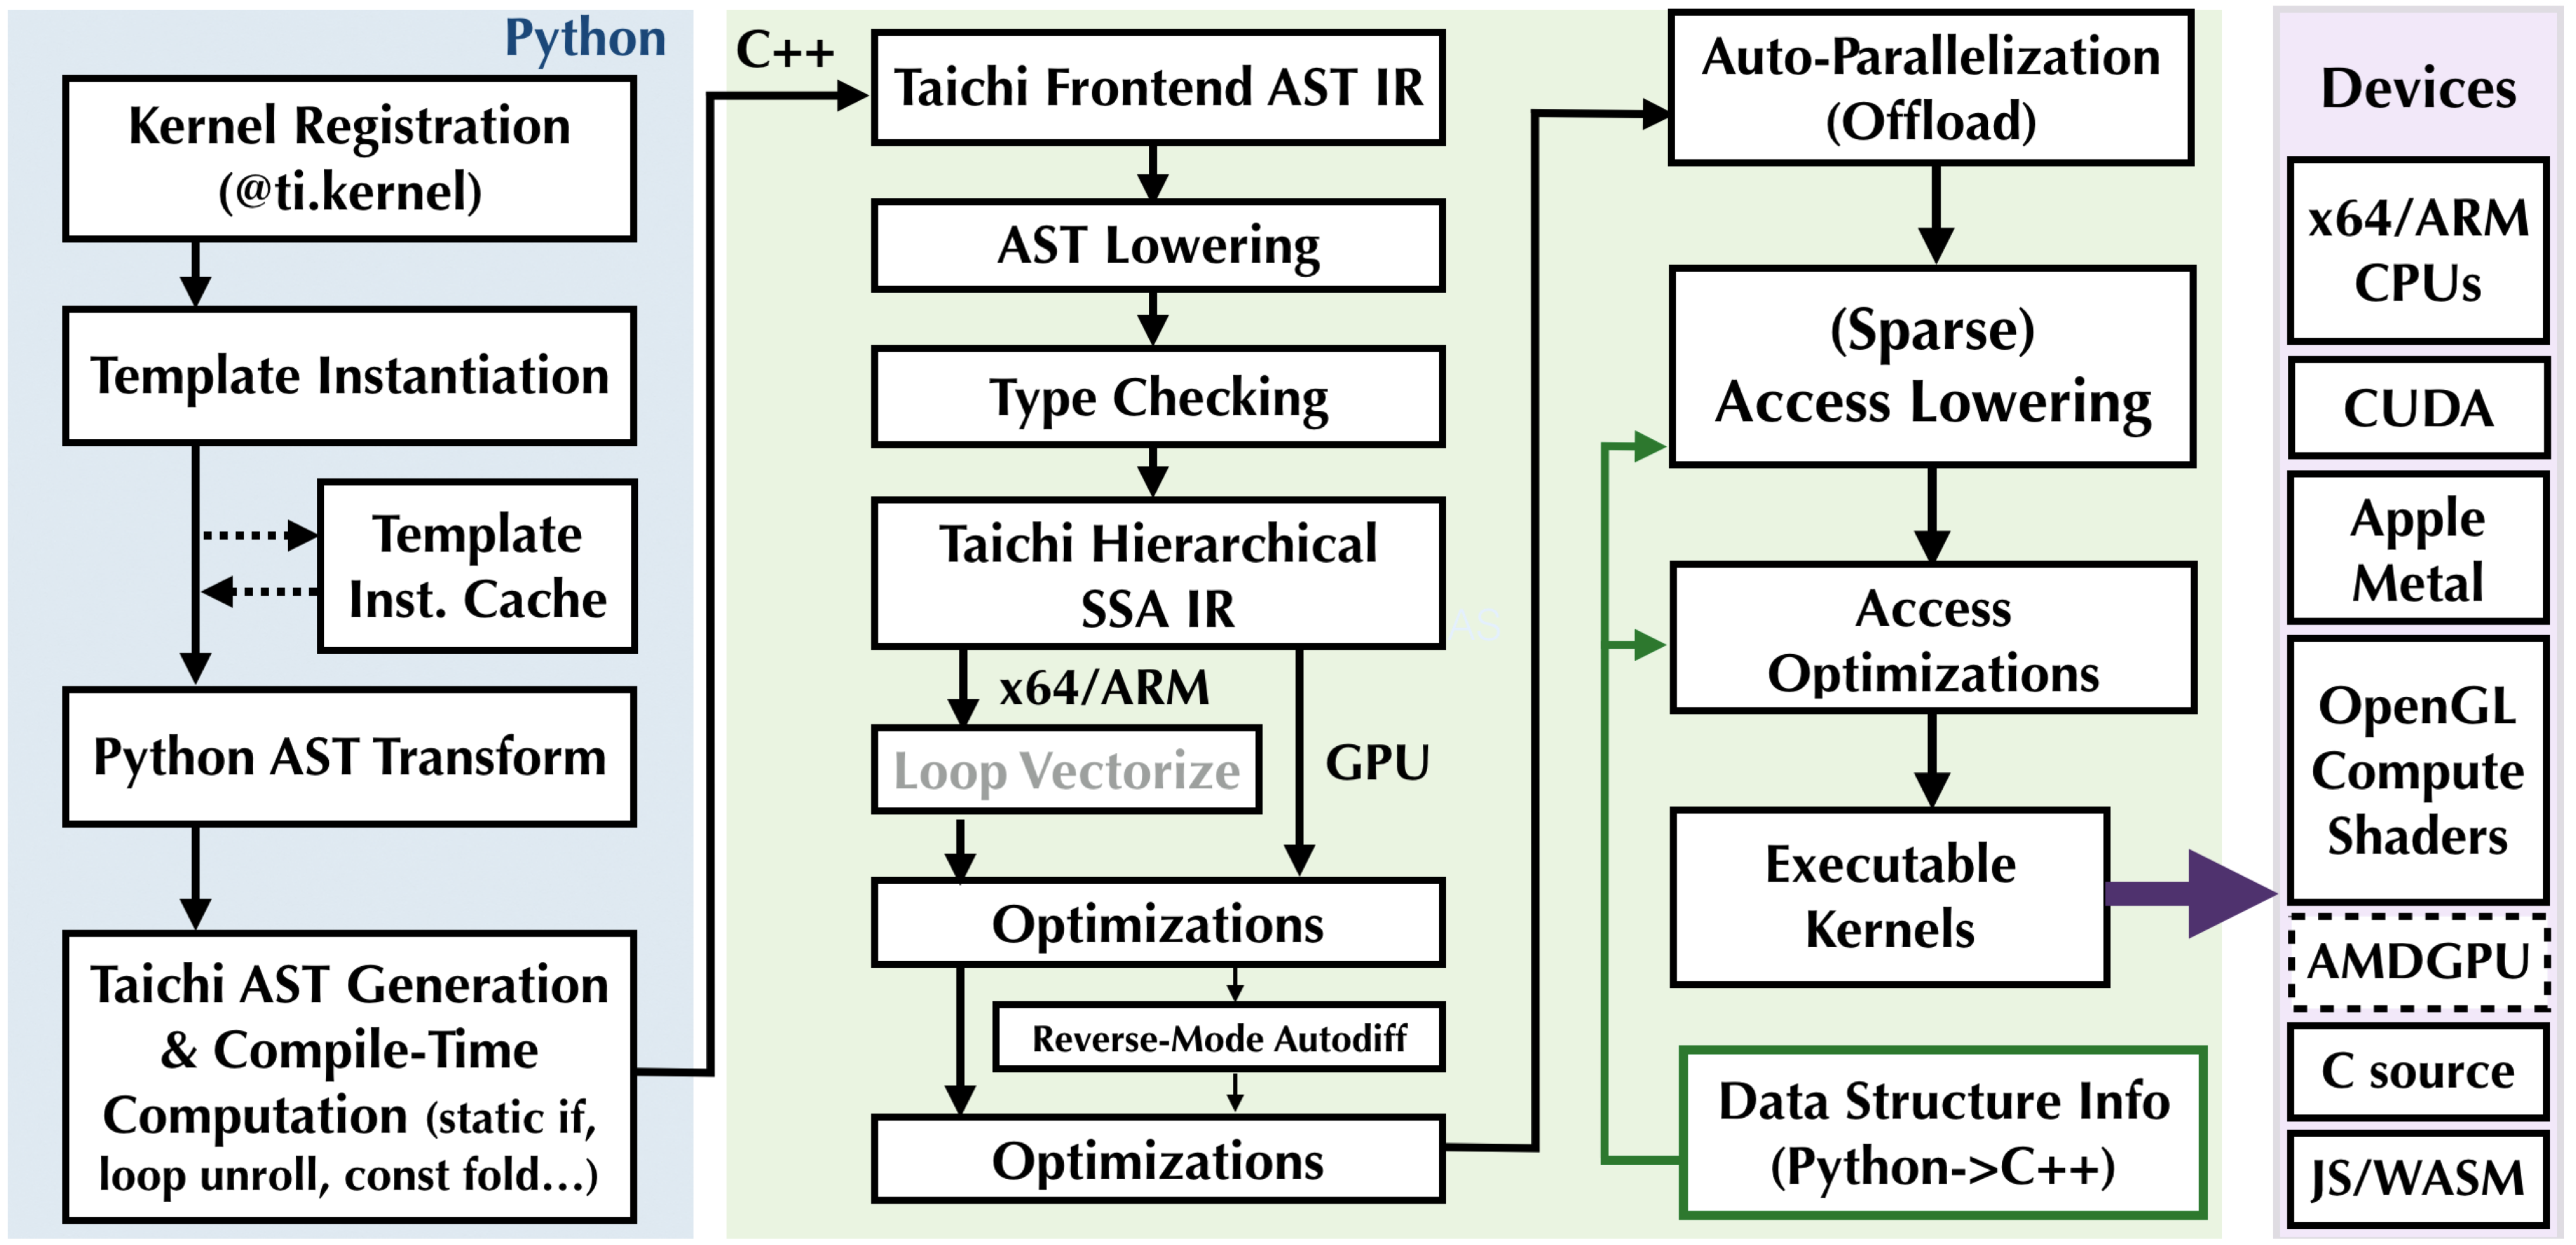
\includegraphics[width=11cm]{life_of_a_taichi_kernel.png}
  \end{centering}
\end{frame}

\begin{frame}{Why}
  \begin{outline}
    \1 Solution to a difficult area in programming 
      \2 Recreate state-of-the-art solutions 
    \1 Grown into a more general purpose tool
      \2 A fantastic edition to the python ecosystem 
      \2 Growing ecosystem (documentation, profiler, ect)
    \1 Creative Coding
      \2 Has some similarities to \href{https://processing.org}{Processing}
  \end{outline}
\end{frame}

\begin{frame}{History}
  \begin{outline}
    \1 Published ACM Transactions on Graphics 2019 \cite{Hu2019}
    \1 \href{https://yuanming.taichi.graphics/publication/2021-taichi-thesis/}{Thesis (MIT)} 
    completed in 2021
  \end{outline}
\end{frame}

\begin{frame}{Workflow}
  \begin{outline}
    \1 Write Kernels in python
    \2 Compiler 
  \end{outline}
\end{frame}

\begin{frame}{Octree}

\end{frame}

\begin{frame}{What is OpenVDB?}
  \begin{outline}
    \1 Published in ACM Trans. Graphics 2013 \cite{Museth2013}
    \1 Work was completed at Dreamworks animation
    \1 Widely used for special effects and animation
      \2 Supported by industry standard software like Houdini and Blender
  \end{outline}
\end{frame}

\begin{frame}{How does OpenVDB Work?}

\end{frame}

\begin{frame}{SPGrid}
  \begin{outline}
    \1 Published in ACM Trans. Graphics 2014 \cite{Setaluri2014}
  \end{outline}
\end{frame}

\begin{frame}[allowframebreaks]{References}
\tiny
\printbibliography
\end{frame}


